\chapter{Security}

\section{Fundamentals}

\subsection{Bedrohungen}
Bedrohungen sind vielschichtig:
\begin{multicols}{2}
\begin{itemize}
	\item Unsichere Konfiguration	
	\item Schwache Protokolle
	\item Implementations-Fehler
	\item Komplexität
	\item Ungenügende Berücksichtigung der Security im Design
\end{itemize}
\end{multicols}

\noindent Es gibt unterschiedliche Angriffstechniken:
\begin{multicols}{2}
\begin{itemize}
	\item Viren/Würmer
	\item Trojan Horse
	\item DoS/DDos
	\item Session Hijacking
	\item Man-in-the-middle
	\item Spoofing
	\item Cross Site scripting
	\item Böse / unwissende Mitarbeiter
\end{itemize}
\end{multicols}

\subsection{Security Konzepte}
Den Bedrohungen kann auf unterschiedliche Art- und Weise begegnet werden:
\begin{description}
	\item[Identification:] Dabei geht es nur darum, wer man ist. Bei einem Gespräch sage ich: 'Hallo, ich bin Bruno'. Somit habe ich mich als Bruno identifiziert. Dabei geht es nicht um die Verifikation ob das auch stimmt, denn das ist Teil der Authentication.
	
	\item[Authentication:] Verifikation, dass derjenige wirklich der ist, den er angibt. Der Authentication-Prozess beginnt in der Regel mit dem Identification-Prozess.
	
	\item[Authorization:] Prüfung der Rechte. Definiert wer was im System machen kann.
	
	\item[Confidentiality:] Daten müssen vertraulich behandelt werden. Sensitive Informationen dürfen nicht in die falschen Hände gelangen. Aber die richtigen Leute müssen an die Daten kommen!
	
	\item[Integrity:] Im Zentrum stehen die Daten. Die Integrität muss über den gesamten Lebenszyklus gewährleistet sein. Keine unberechtigten Personen dürfen die Daten mutieren können. Auch beim Absturz von Diensten oder anderen nicht-menschlichen Einflüssen darf die Integrität nicht beeinträchtigt werden.
	
	\item[Administration:] Ein klares Administrations-Konzept ist wichtig.
	
	\item[Auditing:] Protokollierung der Aktivitäten der Benutzer.
	
	\item[Program Robustness:] Programme müssen robust implementiert sein, damit diese beim Fehlerfall nicht irgendwelche unerwünschte Dinge preis geben.
	
	\item[Configuration Mgmt.:] Auf welchem System, welches Artefakt in welcher Version installiert ist, dient dazu um seine Landschaft im Griff zu haben.
	
	\item[Benutzer-Schulung:] Das schwächste Glied in Kette stellt oft der Mensch selbst dar. Diese müssen im Umgang mit den Informatik-Instrumenten geschult werden.
\end{description}

\subsection{Security Technologien}
\begin{multicols}{2}
\begin{itemize}
	\item Cryptography
	\item Public Key Infrastructure (PKI)
	\item XML Security Specifications
	\item Authentication Servers/SSO
	\item Transport Layer Security (TLS/SSL)
	\item Firewalls
	\item Anti-Virus Software
	\item Intrusion Detection Systems
	\item Vulnerability Analysis Tools
	\item Virtual Private Networks
\end{itemize}
\end{multicols}


\section{Java Platform Security}

\subsection{Sprachmodell}
Das Ziel von Java ist, dass Anwendungen eine sichere Plattform bekommen. Dabei wurde bereits auf Stufe des Sprachmodell gewisse Entscheidungen dafür getroffen:
\begin{itemize}
	\item Keine Pointer sondern Objektreferenzen
	\item Virtuelle Maschine - überwachte Ausführung und Rechte
	\item Strenge Typisierung
	\item Sichtbarkeiten (private, protected, package, public)
	\item Kontrollierte Programmabbrüche mittels Exceptions
	\item Strenge Array-Grenzen - Zugriff auf benachbarte Elemente nicht möglich
\end{itemize}

\subsection{Security Flow}
\begin{figure}[h!]
\centering
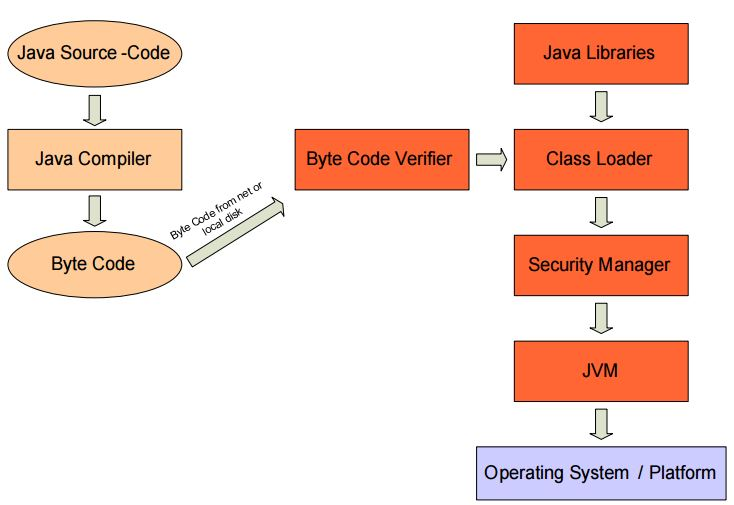
\includegraphics[width=0.5\linewidth]{fig/java-security-flow}
\caption{Java Security Flow}
\label{fig:java-security-flow}
\end{figure}

\subsubsection{Byte Code Verifier}
Der Bytecode soll nach Kompilation unverändert bleiben. Der Byte Code Verifier prüft vor Ausführung alle Class-Files ausser die des JDKs. Mittels \verb|java -noverify| kann diese Prozess deaktiviert werden - logischerweise nicht zu empfehlen. Dafür gibt es vier sogenannte \emph{Pass}:
\begin{description}
	\item[Pass 1 - Format:] Der Java Interpreter prüft zuerst das Format des Class-File. Beispielsweise muss es immer mit \verb|0xCAFEBABE| beginnen.
	
	\item[Pass 2 - Java-Konzepte:] Prüft ob  die Konzepte von Java eingehalten sind. Dies umfasst Vererbungshierarchien, gültige Objekt-Verweise, Variablen müssen vor ihrer Benutzung initialisiert werden, auf private Daten und Methoden kann nur innerhalb der Klasse zugegriffen werden und noch viele weitere.
	
	\item[Pass 3 - Programmausführung:] Datenflussanalyse der Methode während dem Linken.
	
	\item[Pass 4 - Referenzen:] Verweise auf fremde Klassen, Methoden und Attribute während dem dynamischen Linken.
\end{description}

\subsubsection{Class Loader}
Nach der Verifikation des Byte Codes werden die Klassen geladen. Dabei gibt es drei Arten wie Klassen sicher geladen werden können:
\begin{description}
	\item[Class Loader und Namespaces:] Der Class Loader ist zuständig für das Laden von Klassen. Der built-in Class Loader von Java wird \emph{primordial class loader} genannt. Es können auch eigene Class Loader implementiert werden. Der Class Loader muss die Namespaces schützen. Beispielweise kann ich nicht einfach eine eigene Klasse in das Package \verb|java.lang| in meinem Projekt implementieren. Erstens könnte ich ja bestehende Klassen so überschreiben oder auf package-private Ressourcen zugreifen. Der \emph{primordial class loader} wirft in diesem Fall eine \verb|SecurityException|.
	
	\begin{figure}[h!]
	\centering
	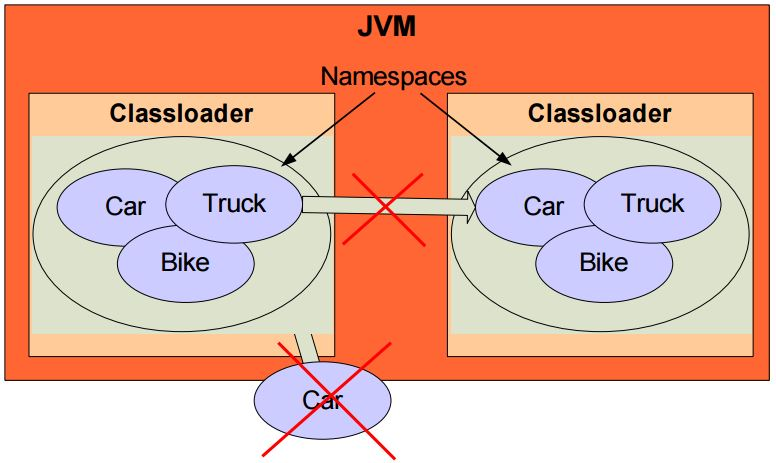
\includegraphics[width=0.7\linewidth]{fig/java-platform-namespaces}
	\caption{Classloader and Namespaces}
	\label{fig:java-platform-namespaces}
	\end{figure}

	\item[Trusted Class Libraries:] Die Class Loaders bilden eine Hierarchie. Die System-Klassen (JDK) sind trusted.
	\begin{figure}[h!]
	\centering
	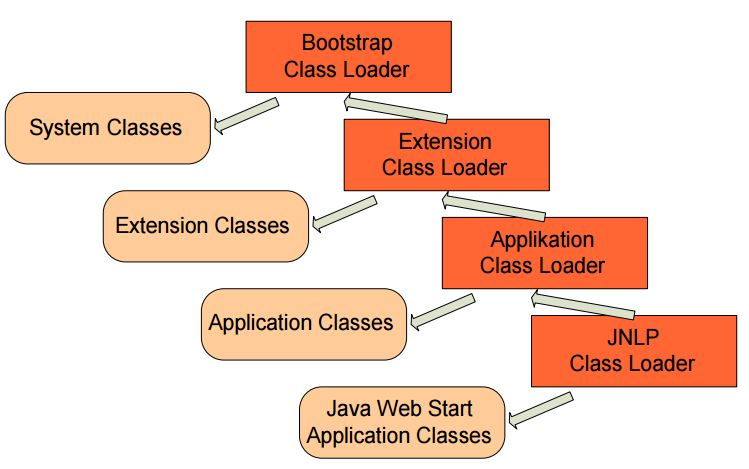
\includegraphics[width=0.5\linewidth]{fig/java-classloader-trusted-libraries}
	\caption{Classloader and trusted libraries}
	\label{fig:java-classloader-trusted-libraries}
	\end{figure}

	\item[Protection Domains:] Jede Klasse wird einmalig bei ihrer Erzeugung einer Protection Domain zugeordnet. Eine Protection Domain ist eine Zuordnung von Rechten zu bestimmten Code (CodeSource, Principal). Kann während der Lebenszeit einer Klasse nicht mehr geändert werden. Kapselt CodeSource, Principal array, ClassLoader und PermissionCollection.
\end{description}

\subsection{Sandbox}
Nicht vertrauenswürdiger Code kann nur innerhalb der Sandbox agieren.
\begin{figure}[h!]
\centering
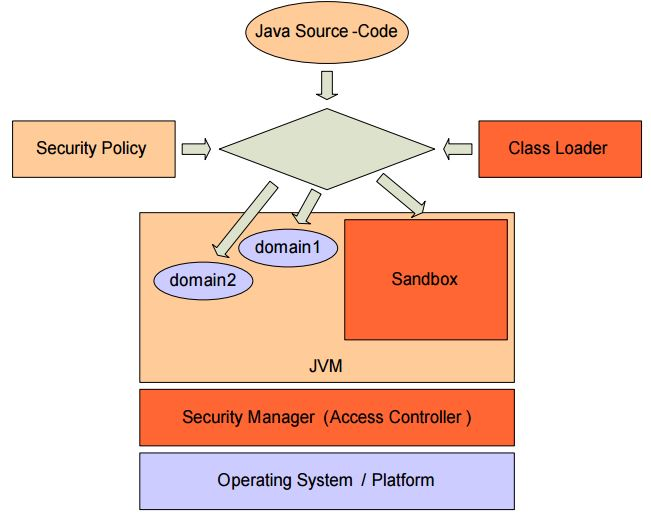
\includegraphics[width=0.7\linewidth]{fig/java-sandbox}
\caption{Sandbox}
\label{fig:java-sandbox}
\end{figure}

Folgendes ist untersagt:
\begin{itemize}
	\item File/Directory-Zugriff
	\item Netzwerkzugriff
	\item Benutzerinfo abfragen
	\item Programme ausführen oder dynamisch Bibliotheken laden
	\item Class Loader / Security Manager instanzieren
	\item Threads kreieren oder manipulieren (ausserhalb ThreadGroup)
	\item Klassenzugriff ausserhalb Package 
\end{itemize}

\subsection{Security Manager}
Der Security Manager prüft ob die Applikation die entsprechende Rechte hat um die Aktionen durchzuführen. Wenn der Security Manager aktiviert ist, ist alles gesperrt, was es zu sperren gibt. Beim Ausführen eines Java-Programmes kann folgendes mitgegeben werden um diesen zu aktivieren: \verb|-Djava.security.manager -Djava.security.policy=java.policy|. Im Policy-File müssen die entsprechende Permissions definiert werden, was die Applikation alles darf. Die Performance leidet darunter natürlich etwas. Einige Beispiele:

\begin{multicols}{2}
\begin{itemize}
	\item java.io.Permission
	\item java.util.PropertyPermission
	\item java.net.SocketPermission
	\item java.lang.RuntimePermission
\end{itemize}
\end{multicols}

\begin{lstlisting}
grant {
	permission java.util.PropertyPermission "user.home", "read";
};
\end{lstlisting}

\subsection{Jar-Signierung}
Jars können signiert werden: \verb|jarsigner enapp_ee_security_uebung01.jar .hsluKeystore|. Dabei werden Public-Key und das Zertifikat in das Jar miteingepackt. Benutzer des Jars können dann das Jar verifizieren.

\section{JAAS}
Bisher haben wir mit der Java Platform Security ein \emph{codezentriertes Sicherheitsmodell} gesehen, welches die Herkunft des Codes die Zugriffskontrolle sicherstellt. Die Java Platform Security wird durch JAAS (Java Authentication and Authorization Service) erweitert, welches ein \emph{benutzerzentriertes Sicherheitsmodell} darstellt. JAAS ist für Multiuser-Applikationen wichtig und die Standardimplementierung des JEE-deklarativen Sicherheitsmodell.

\subsection{JAAS-Objects}
Benutzer können sowohl Personen wie auch Dienste (Subjects) sein. Davon kann jedes mehrere Identitäten (Principal - Name, Email, Kreditkartennummer) und Berechtigungen (Credentials - Passwort, Zertifikat, Keys) besitzen. 

\subsection{JAAS-Architecture}
JAAS stellt schlussendlich nur APIs zur Verfügung und zwar für beide Seiten. Zum einem für die Applikations-Entwickler und zum anderen für Security-Softwarehersteller. Für zweiteres stellt JAAS sogenannte SPIs zur Verfügung, welche implementiert werden können. So kann ich das Login Modul austauschen von Kerberos auf LDAP oder vielleicht auf Smartcard.

\section{Java EE Security}
Java EE ist eine Plattform für die Entwicklung von verteilten Systemen. Das Design der Plattform ist dabei auf die Entwicklung und das Deployment von \emph{sicheren} Systemen ausgelegt. Trotzdem sind noch längst nicht alle Security-Themen adressiert. Es beinhaltet sichere und robuste API's sowie SPI's (service provider interface) für die Produktehesteller von Sicherheitslösungen. Sowie Sicherheits-Konfiguration zur Deployment Zeit. Es sollen folgende Ziele erreicht werden:

\begin{description}
	\item[Portabilität:] 'Write once, run everywhere'
	\item[Transparenz:] Applikationsentwickler müssen keine tiefgründigen Kenntnisse über Security haben um ihre Applikationen zu	entwickeln.
	\item[Isolation/ Abstraktion:] Trennung von Business und Security –	Der Deployer kann die Sicherheit hinzufügen.
	\item[Erweiterbarkeit:] Die Portabilität der Applikation wird durch die	Einbindung von Sicherheits-Services nicht behindert.
	\item[Unabhängigkeit:] Die Einbindung von verschiedenen	Sicherheitstechnologien soll möglich sein.
\end{description}

\begin{figure}[h!]
\centering
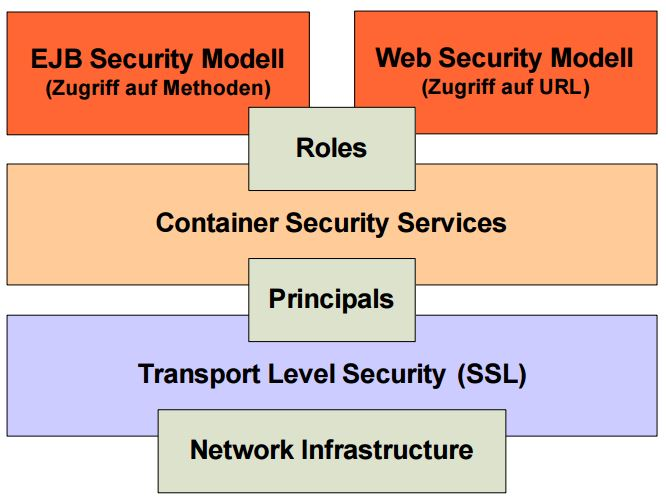
\includegraphics[width=0.7\linewidth]{fig/java-ee-security}
\caption{Java EE Security Architecture}
\label{fig:java-ee-security}
\end{figure}

Die Rollen werden gemappt. Ein Java EE Entwickler kann seine eigenen Rollen in der Applikation definieren. In einem Konfigurations-File können die Rollen zu den konkreten Rollen gemappt werden. Dieses Mapping ist oft auch Herstellerspezfisch. Das Mapping von LDAP zu JavaEE Rollen sieht vielleicht anders aus als bei Kerberos.

Es wird zwischen \textbf{deklarativer Security} und \textbf{programmatischer Security} unterschieden. Ersteres definiert wer beispielsweise auf welches EJB und dessen Methoden zugreifen kann, dies aber nur grob-granular. Die Methode \verb|getUser| kann von der Rolle \verb|Guest| ausgeführt werden, jedoch kann \verb|deleteUser| nur von \verb|Admin| ausgeführt werden. Bei der programmatischen Security schreibe ich Programmcode, welches auf den Principal (Idendity) zugreift und basierend auf diesem Entscheidungen fällt. Beispielweise kann ich den Beitrag nur editieren, wenn ich der Ersteller des Beitrages bin.

Der \textbf{Realm} ist eine 'komplette' Datenbank mit Benutzern und Gruppen. Der Realm kann also valide User einer Applikation identifizieren. Es gibt: File-Realm, Certifcate-Realm, LDAP-Realm usw.


\subsection{Java EE - Authorization}
Die Authorization-Mechanismen können sowohl im \emph{Web Tier} wie auch im \emph{EJB Tier} verwendet werden. Logischerweise können hier \emph{deklarative} und \emph{programmatische} Sicherheitsimplementation gemeinsam benutzt werden. Es wird zwischen vier Szenarien unterschieden, welche jede Kombination aus Web-Tier und EJB-Tier mit deklarativer und programmatischer Security vereint.

\paragraph{Web-Tier}
Mit deklarativer Security kann der Zugriff auf Web Ressourcen reguliert werden, welche im \verb|web.xml| oder als Annotationen definiert werden. Diese Regeln werden durch den Web-Container umgesetzt. Fein-granulare Zugriffsteuerung ist jedoch nicht möglich, nur auf Basis der Klasse (\emph{Anmerkung Autor: Ich glaube diese Aussage ist falsch. Im Servlet kann ich auf Stufe Methode annotieren}?). Programmatisch kann im Servlet, im JSP oder im JSF eingegriffen werden. 

\paragraph{EJB-Tier}
Mit deklarativer Security kann der Zugriff auf Beans und Methoden reguliert werden, welche im \verb|ejb-jar.xml| oder als Annotationen definiert werden. Die Regeln werden durch den EJB-Container umgesetzt. Feine granulare Zugriffsteuerung ist möglich auf Stufe Methode. Programmatisch kann direkt im EJB Einfluss genommen werden.

\paragraph{Vorgehen im EJB-Tier}
\begin{enumerate}
	\item Der Deployer definiert die Rollen im Deployment Deskriptor (kann auch über Annotationen im Code hinterlegt werden).
	
	\item Anschliessend werden die Zugriffsrechte der Business-Methoden zu den Rollen zugewiesen (Deployment-Deskriptor oder Annotationen).
	
	\item Zum Schluss wird das Mapping der Gruppen zu den deklarierten Rollen im herstellerspezifischen Deployment Deskriptor definiert.
\end{enumerate}

\newpage

Listing \ref{lst:deklarative-security} zeigt wie deklarative Security im EJB-Tier umgesetzt wird. Es wird die Möglichkeit mit XML und mit Annotationen gezeigt.

\begin{lstlisting}[caption=Deklarative Security im EJB-Tier, label=lst:deklarative-security]
// Schritt 1 - Deployment Deskriptor
<enterprise-beans>
	<assembly-descriptor>
		<security-role>
			<description>People manages other people</description>
			<role-name>manager</role-name>
		</security-role>
		<security-role>
			<description>People who are employeed</description>
			<role-name>employee</role-name>
		</security-role>
	</assembly-descriptor>
	...

// Schritt 1 - Alternativ als Annotation
@Stateless
@DeclareRoles({"manager", "employee"})
public class StatelessSessionBean implements StatelessSession {

// Schritt 2 - Deployment Deskriptor
<assembly-descriptor>
	<method-permission>
		<role-name>manager</role-name>
		<method>
			<ejb-name>StatelessSessionBean</ejb-name>
			<method-name>getSalary</method-name>
		</method>
	</method-permission>
</assembly-descriptor>

// Schritt 2 - Alternativ als Annotation
@RolesAllowed("manager")
public String getSalary(String name) {

// Schritt 3 - Rollen-Mapping
<security-role-mapping>
	<role-name>manager</role-name>
	<group-name>g_manager</group-name>
	<role-name>employee</role-name>
	<group-name>g_employee</group-name>
</security-role-mapping>
\end{lstlisting}

Annotationen sind gut geeignet für einfachere Applikationen - übersichtlich und direkt im Code sichtbar. Für umfangreichere Applikation ist die Verwendung der Deployment-Deskriptoren besser geeignet. Die Konfiguration ist ersichtlich ohne, dass im Code nachgeschaut werden muss \emph{(Anmerkung Autor: Ich bin nicht dieser Meinung)}. Listing \ref{lst:programmatische-security} zeigt wie die programmatische Security im EJB-Tier umgesetzt wird.

\newpage

\begin{lstlisting}[caption=Programmatische Security im EJB-Tier, label=lst:programmatische-security]
// Schritt 1: Programmieren

public double getSalary(String employeeId) {
	java.security.Principal p = ctx.getCallerPrincipal();
	String callerId = p.getName();
	// "manager" role can read employee salary information
	// employee can read only his/her own salary information
	if ((ctx.isCallerInRole("manager")) || ((ctx.isCallerInRole("employee")) && (callerId == employeeId))) {
		// return Salary information for the employee
		return getSalaryInformationSomehow(employId);
	} else {
		throw new SecurityException("access denied");
	}
}

<!-- Schritt 2: Abstrakte Security Rolle -->
<security-role-ref>
	<description>abstract manager role</description>
	<role-name>manager</role-name>
<security-role-ref>

<!-- Schritt 3: Abstrakte Security Rolle mappen -->
<security-role-ref>
	<role-name>manager</role-name>
	<role-link>managerOfHSLU</role-link>
</security-role-ref>
<assembly-descriptor>
	<!-- Deployer declared real security roles -->
	<security-role>
	<description>real manager role in HSLU</description>
	<role-name>managerOfHSLU</role-name>
	</security-role>
</assembly-descriptor>
\end{lstlisting}

\subsection{Java EE - Authentication}
Authentication ist Aufgabe des EJB-Containers und muss nicht implementiert werden. Authentication ist Container-spezifisch: Username/Passwort, X.509, Kerberos. Programmatische Authentication wird nicht unterstützt. Es gibt zwei Optionen:

\begin{description}
	\item[Option 1:] Informationen des Benutzers (UserId, Passwort, Zeritifkate, usw.) im Web-Tier ermitteln und an die eigentliche Authentifizierung an den EJB-Tier weiterleiten. 
	\item[Option 2:] (Best Practice): Im Web-Tier werden die Informationen ermittelt und die Authentifizierung auch gleich durchgeführt. Der Web-Tier leitet die Identity des Benutzer in Form einer Principal-Instanz an den EJB-Tier weiter. 
\end{description}

Was ist aber, wenn wir keinen Web-Tier dazwischen haben und ein Client sich direkt gegen einen EJB-Container authentifizieren soll? Dafür könnte man ein JAAS-Login machen oder besser einen Client-Container verwenden, welcher aber herstellerspezifisch ist (best practice). Dabei muss der Client-Container die User Credentials ermitteln und den Benutzer gegen den EJB Server authentifizieren. Der Client-Container wrappt die den EJB-Client und wird zum Deployment-Zeitpunkt instanziert.

\emph{P.S: EIS heisst Enterprise Information Layer. Und wird bei Zeichnungen oft nach dem EJB-Tier dargestellt.} 